\documentclass[11pt]{article} 
\usepackage[utf8]{inputenc}
\usepackage{amstext}
\usepackage{amsmath}
\usepackage{graphicx}
\usepackage{textcomp}
\usepackage{float}
\usepackage{varioref}
%\usepackage{fancyref}
\usepackage{caption}
\usepackage{subcaption}
\usepackage{comment}
\usepackage{hyperref}
\usepackage{epstopdf}
\usepackage[margin=1in, paperwidth=8.5in, paperheight=11in]{geometry}
\usepackage{listings}
\usepackage{color}

\pdfpageattr {/Group << /S /Transparency /I true /CS /DeviceRGB>>} 

\definecolor{dkgreen}{rgb}{0,0.6,0}
\definecolor{gray}{rgb}{0.5,0.5,0.5}
\definecolor{mauve}{rgb}{0.58,0,0.82}

\lstset{frame=tb,
  language=Java,
  aboveskip=3mm,
  belowskip=3mm,
  showstringspaces=false,
  columns=flexible,
  basicstyle={\small\ttfamily},
  numbers=none,
  numberstyle=\tiny\color{gray},
  keywordstyle=\color{blue},
  commentstyle=\color{dkgreen},
  stringstyle=\color{mauve},
  breaklines=true,
  breakatwhitespace=true
  tabsize=3
}

\vrefwarning

\title{Real World Measurements Final Project Report}
\author{Jay Woo, Sidd Singal, Filippos Lymperopoulos, James Jang}
%\date{Now} 

\begin{document}
\maketitle
\vspace*{45 mm}
\begin{abstract}
The goal of our Real World Measurements final project was to accurately map the heat signature of a specific test object. The circuit implemented was relatively simple, yet the programming and mechanical design were very involving. We produced a relatively decent heatmap using the Arduino microcontroller. 
\end{abstract}
\newpage

\section{Background Information}

Every person and object emits some amount of infrared radiation. Through infrared thermography, one can develop a "camera" that captures a specific heat signature. Hot objects are often depicted as red pixels, while cold objects are depicted as blue pixels.

The infrared spectrum is characterized as an electromagnetic range of wavelengths varying between 9$\mu$m and 14 $\mu$m. Hence, the infrared radiation of an object increases proportionally with the magnitude of the temperature it is characterized by.

Using the proper sensor, we can collect temperature data at long distances. After combining these data points, we can produce a thermal image, also called a thermogram. At each pixel, the generated image displays the amount of infrared radiation that is being emitted from that particular point.

An example of a heat map depicting buildings and their temperature variations is given below in Figure 1.

\begin{figure}[!ht]
	\centering
	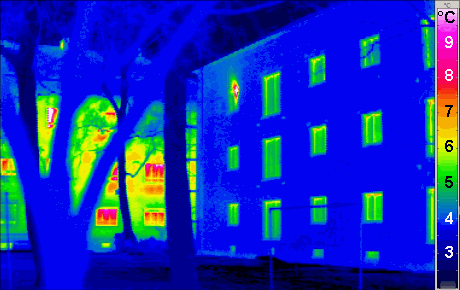
\includegraphics[width=.8\textwidth]{example}
	\caption{Example of thermogram depicting buildings and their temperature changes}
	\label{fig:cover}
\end{figure}

It should be noted that the analysis of heat signatures in buildings can be extremely useful for examining energy use distribution. Heat maps provide important information on heat losses, as well as the rate of temperature decay, of various objects.

\newpage
\section{Parts List}
This is a list of all the parts we bought, along with their respective prices.

\begin{itemize}
	\item $\bf Arduino$ $\bf Uno$ microcontroller, Price: N/A
	\item $\bf Two$ $\bf DC$ $\bf Geared$ $\bf Servo$ $\bf Motors$ $\bf 6V$ - Parallax Inc. 900-00008, Price: \$27.98
	\item $\bf Two$ $\bf DC$ $\bf Servos$ $\bf 4.8V$ - $\bf 6V$ - TowerPro SG-5010, Price: \$24.00
	\item $\bf Two Temperature$ $\bf Sensors$ - Melexis MLX90614, Price: \$24.48
	\item $\bf Two$ $\bf Resistors$ - 4.9k$\Omega$ each, Price: N/A
	\item $\bf Capacitor$ - 0.1$\mu$F, Price: N/A
\end{itemize}

\bf{Total Cost}: \$76.46

\section{Circuit Analysis}
\normalfont
The circuit used for the experiment was relatively simple, given that the sensor performs much of the important work for us.  Figure 2 is the schematic of the circuit. A4 and A5 are the analog pins of the Arduino UNO, one of which reads the PWM signal from the MLX sensor. Finally, resistors and a capacitor of the depicted values were used, while the ground and 5V pins are denoted accordingly.

\begin{figure}[!ht]
	\centering
	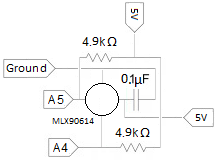
\includegraphics[width=.5\textwidth]{schematic}
	\caption{Schematic of our circuit with the sensor MLX90614}
	\label{fig:cover}
\end{figure}

\section{MLX Sensor}

The following depiction in Figure 3 describes what each pin of the sensor does. Pin 1 is known as the serial clock input for the sensor, and it allows for a master/slave mode of communication. Pin 2 is the PWM output of the sensor. PWM stands for pulse-width modulation - the width of the pulse determines the output value of the sensor. Finally, pin 3 is power, and pin 4 is ground.

\begin{figure}[!ht]
	\centering
	\includegraphics[width=.4\textwidth]{topview}
	\caption{Top view of the MLX90614 infrared sensor}
	\label{fig:cover}
\end{figure}

The MLX90614 sensor has a low noise amplifier built into it, along with a 17-bit ADC, which allow for very accurate and high resolution (to this decimal place - 0.01$^o$C) temperature readings.

We can supply a voltage of 5V to pin 3, VDD, and then pin 2 will act as a digital output/input. We can collect temperature readings from this pin by directly connecting it to the Arduino. We also had to connect one of the Arduino's analog pins to pin 1. In order to communicate with this pin, we had to use a library that we found online (Link: http://bildr.org/2011/02/mlx90614-arduino/).

\section{Integration with the Arduino}
Using the proper circuit diagram, we soldered components onto a piece of protoboard, which we then connected to the Arduino. However, the board didn't have marked traces, so we soldered connections between the various holes, as shown below in Figure 4.

\begin{figure}[!ht]
	\centering
	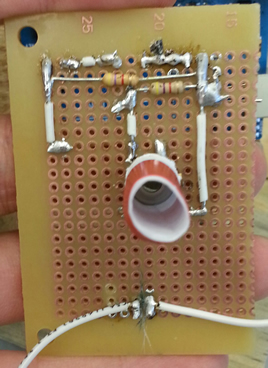
\includegraphics[width=.3\textwidth]{protoboard}
	\caption{A view of the protoboard circuit}
\end{figure}

As it turned out, we couldn't directly control the position of the first two servo motors we bought, Parallax Inc.  900-00008P. As a matter of fact, all we could change was the speed of the servo motors. As an end result, we decided to buy completely different servos, TowerPro SG-5010, which ended up being easier to handle.

In order to manage the position and calibration of the servos,  we decided to use two of the Arduino's digital output pins. In our code, we used a nested for loop to sweep across a range of x and y values. Figure 5 shows a snippet of the code we used to accomplish this.

\begin{figure}[!ht]
    \centering
    \includegraphics[width=\textwidth]{loop}
    \caption{This part of our code simultaneously collects data and controls the servos}
\end{figure}

\section{Mechanical Design}
In order to be able to sweep through a two-dimensional plane, we constructed a mainly wooden mechanism consisting of two servos each moving in a different axis. The first servo was mounted onto the main foundation base and rotated a plate left and right. The other servo rested on top of the plate and faced sideways, to move the sensor up and down. The Arduino board was attached to the second servo, along with the protoboard on which we soldered the sensor. The final product is depicted in Figure 6.

\begin{figure}[H]
    \centering
    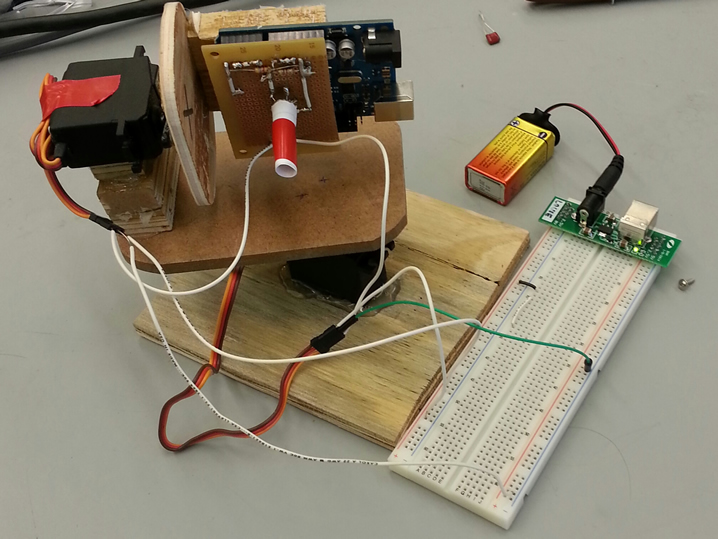
\includegraphics[width=.6\textwidth]{mechdesign}
    \caption{A picture of our mechanical design}
\end{figure}

It is important to note that the Arduino does not have enough power to drive both servos at the same time. Hence, we required a secondary voltage supply, to supply the remaining power. As a result, we connected the servos to a breadboard and powered them with a 5-volt power supply. This was sufficient to power both of them and have them operate effectively.

\section{Experimentation and Results}
We collected data of a person's hand, resting on a wall. We set up the sensor in the following manner (Figure 7):

\begin{figure}[H]
    \centering
    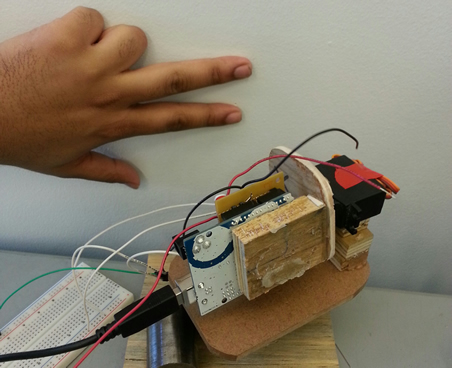
\includegraphics[width=.5\textwidth]{hand.jpg}
    \caption{The hand of one of our brave group members}
\end{figure}

\newpage
We came up with the following result, as given in Figure 8 that follows.

\begin{figure}[H]
    \centering
    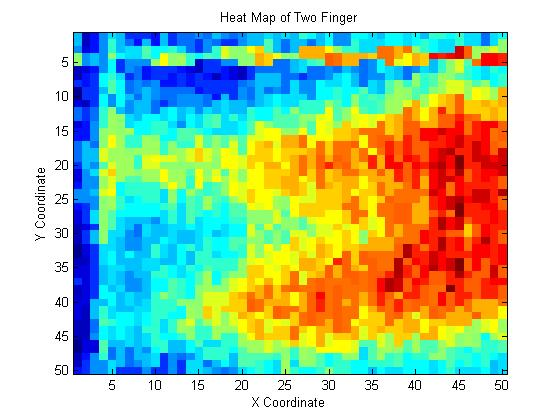
\includegraphics[width=.6\textwidth]{TwoFingers}
    \caption{As shown, the two fingers are clearly outlined in red.}
\end{figure}

We further took a thermal image of a soldering iron, after having it heated up. In Figure 9, the original image is given.
\begin{figure}[H]
    \centering
    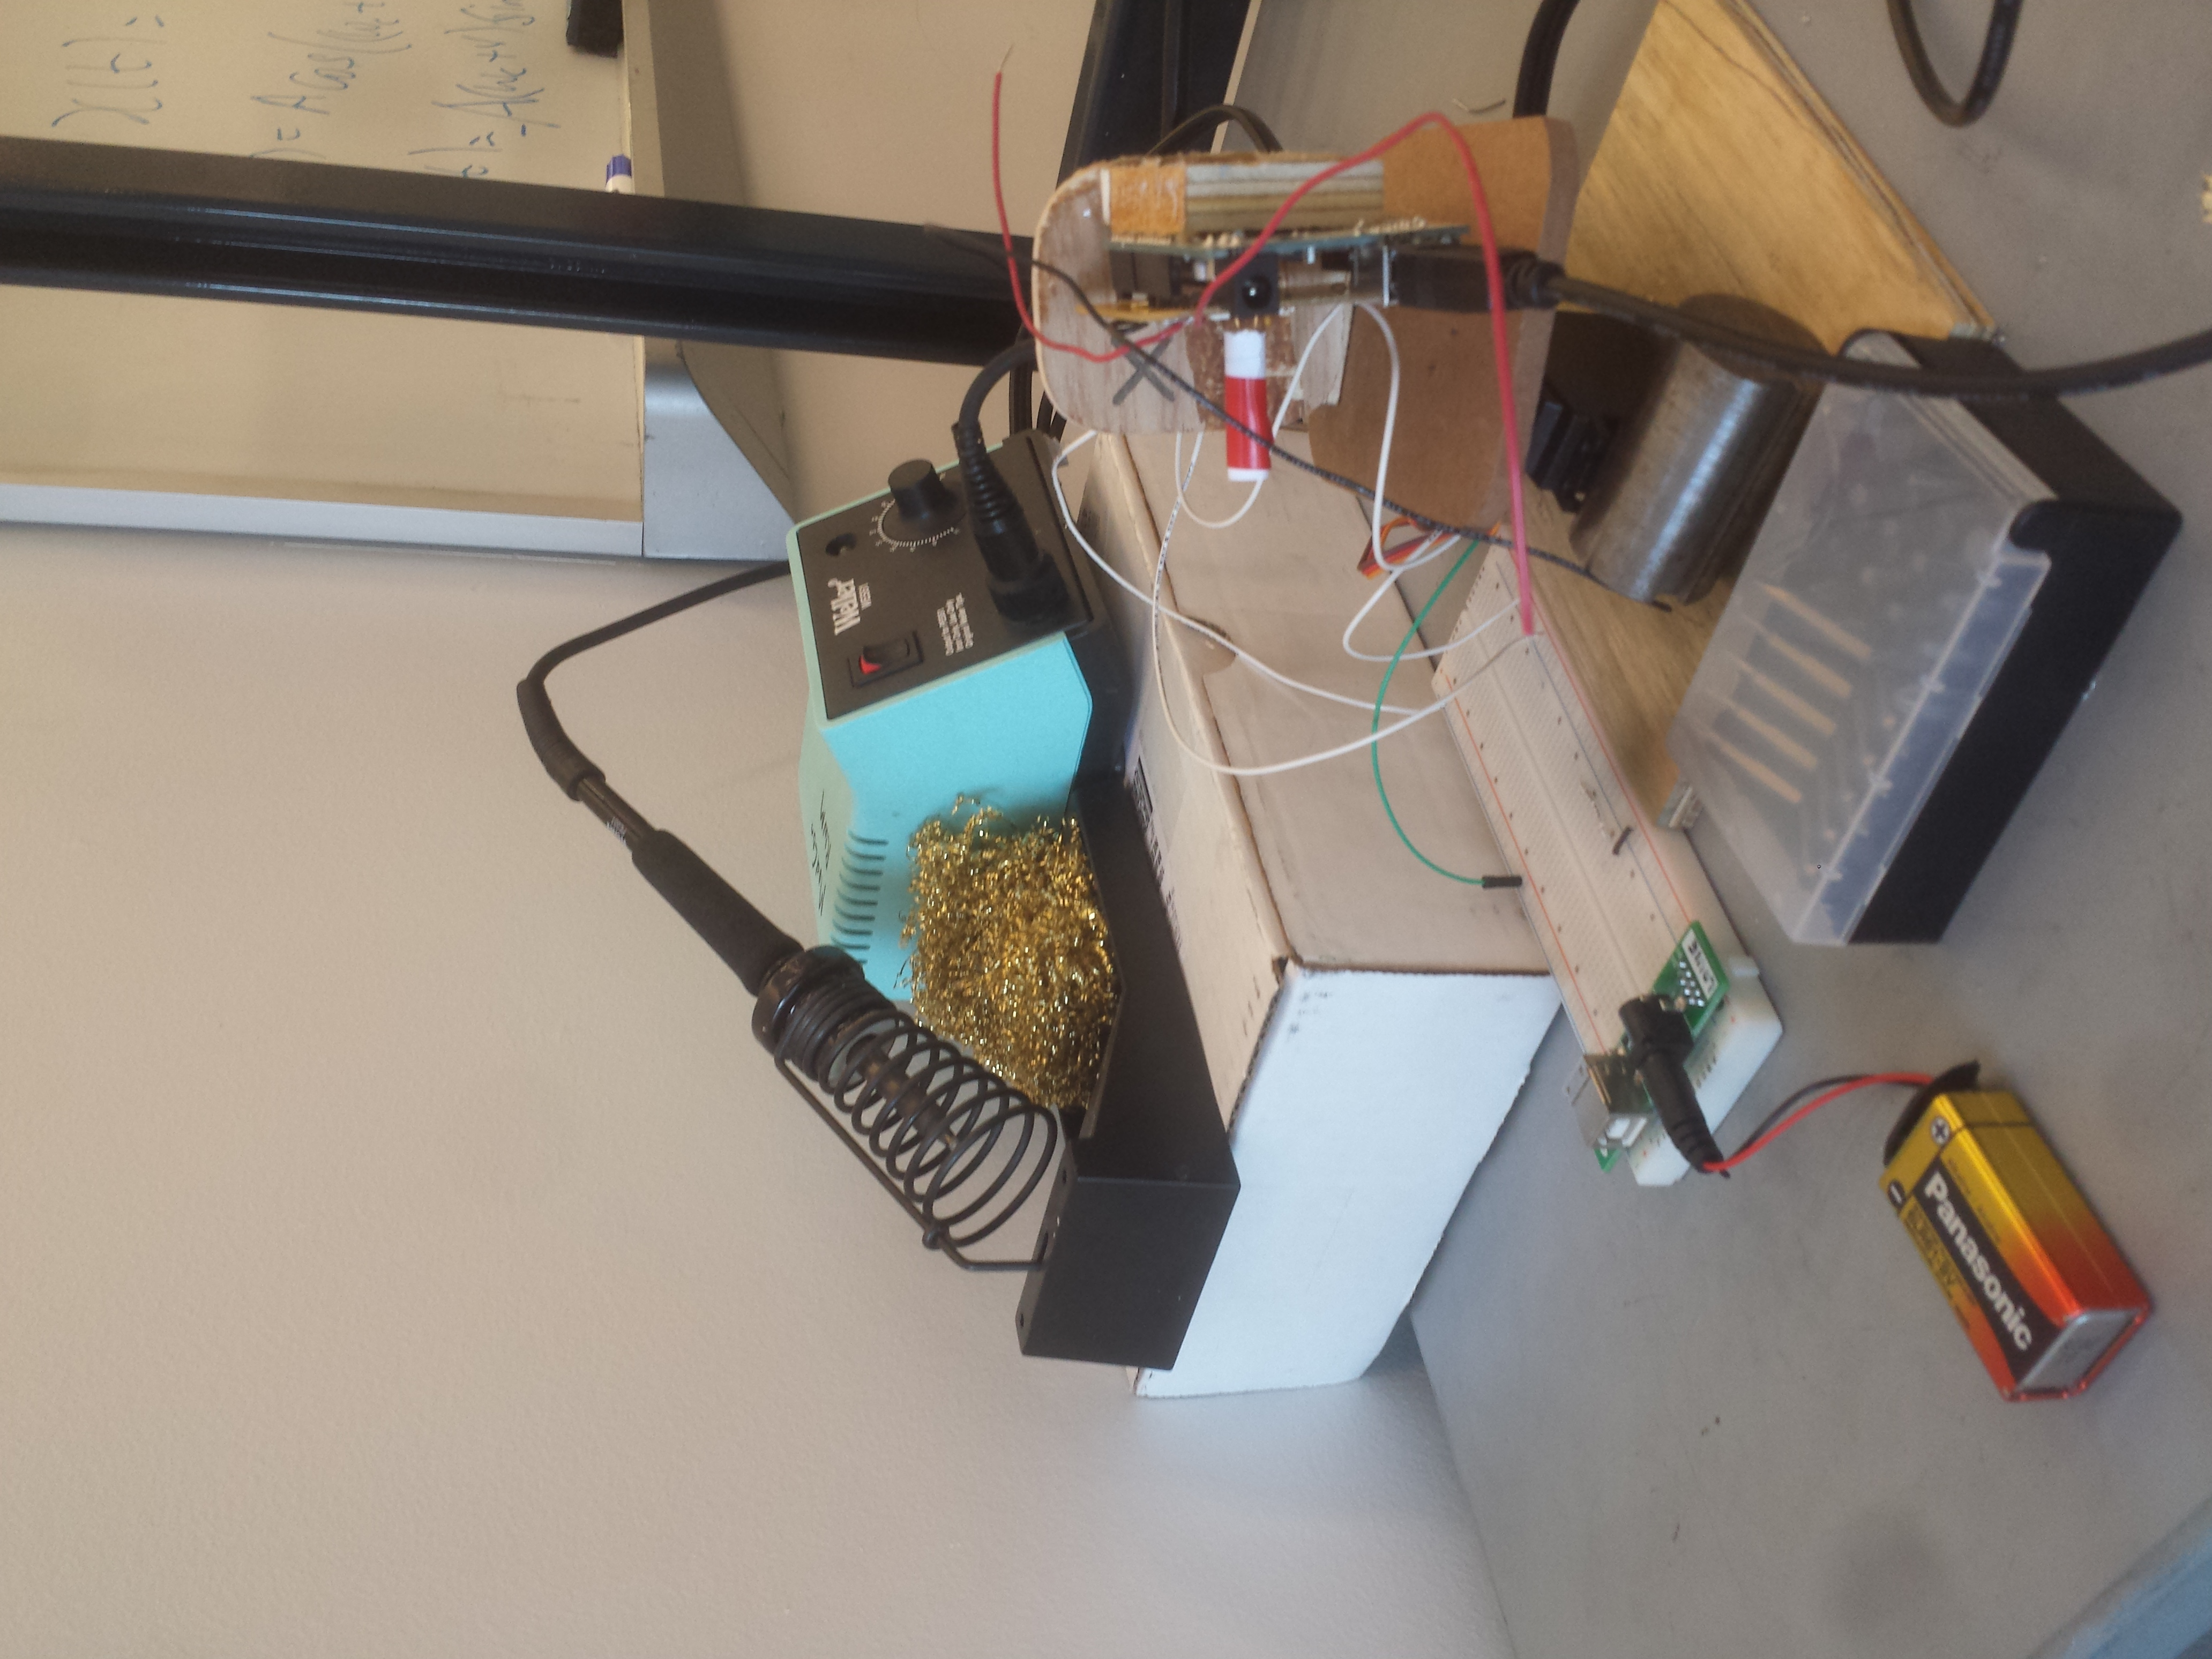
\includegraphics[width=.6\textwidth, angle = 270]{iron}
    \caption{A lonely soldering iron.}
\end{figure}
\newpage

After the scanning of the area and the collection of the data, the following image in Figure 10 is generated.

\begin{figure}[H]
    \centering
    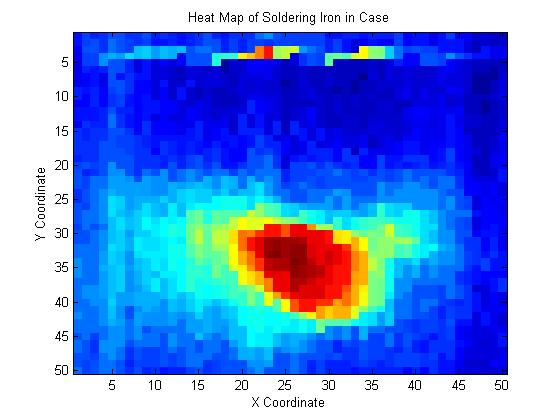
\includegraphics[width=.6\textwidth]{heatmap2}
    \caption{The soldering iron is extremely hot relative to the wall in the background.}
\end{figure}

\section{Results Analysis}

Both thermograms were able to successfully represent heat maps of two fingers and a soldering iron. The two fingers are clearly distinguishable, and the the location of the soldering iron in its case was also identifiable.

One thing to note is that the top of each of the thermograms has a sort of nonsensical noise. This noise was probably created when our thermal camera started taking data before the vertical servo had been reset to the proper starting value. However, these areas can be neglected as their true heat signatures were known (since there was only a wall where heat was suggested).

The outlines of the fingers can be identified for the most part, but it is not perfect. The infrared sensor averages temperatures at a certain point and its surrounding points. This surrounding neighborhood covers too big an area to perfectly depict the outlines of the finger. This can be solved by investing in a more accurate sensor that covers a smaller area.

\newpage
\section{Total Arduino Code}
\begin{lstlisting} 
//Source: http://bildr.org/2011/02/mlx90614-arduino/

#include <i2cmaster.h>
#include <EEPROM.h>
#include <Servo.h>

Servo servoHOR;
Servo servoVER;

void setup(){
  delay(3000);
  Serial.begin(9600);

  i2c_init(); //Initialise the i2c bus
  PORTC = (1 << PORTC4) | (1 << PORTC5);//enable pullups

  servoVER.attach(6);
  servoHOR.attach(7);
  
}

void loop(){
  int counter = 0;     //Stores index of each point of data
  float tempdata;      //Stores temperature data

  for (int currentX = 30; currentX < 80; currentX++) {    //Sweeps through x values b/w 30 and 80
    servoHOR.write(currentX);      //Sets servo to x position
    for (int currentY = 40; currentY < 90; currentY++) {  //Sweeps through y values b/w 40 and 90
      servoVER.write(currentY);    //Sets servo to y position
      delay(10);
      tempdata = get_temp();       //Returns the temperature in Celsius
      Serial.println(tempdata);    //Prints temperature to serial monitor
      counter++;
    }  
    delay(10);
  }
  Serial.end();
  
  while(1) {}                     //Infinite loop that runs after everything is done
}

float get_temp(){
  //INITIALIZATION
  int dev = 0x5A<<1;  //This is the device address of the sensor
  int data_low = 0;
  int data_high = 0;
  int pec = 0;

  //WRITE MODE
  i2c_start_wait(dev+I2C_WRITE); //Sets device address and write mode
  i2c_write(0x07);               //Write value 0x07 to MLX sensor

  //READ MODE
  i2c_rep_start(dev+I2C_READ);   //Sets device address and read mode
  data_low = i2c_readAck(); //Read 1 byte and then send ack
  data_high = i2c_readAck(); //Read 1 byte and then send ack
  pec = i2c_readNak();
  i2c_stop();  

  //This converts high and low bytes together and processes temperature, MSB is a error bit and is ignored for temps
  double tempFactor = 0.02; // 0.02 degrees per LSB (measurement resolution of the MLX90614)
  double tempData = 0x0000; // zero out the data
  int frac; // data past the decimal point

  // This masks off the error bit of the high byte, then moves it left 8 bits and adds the low byte.
  tempData = (double)(((data_high & 0x007F) << 8) + data_low);
  tempData = (tempData * tempFactor)-0.01;


  float celsius = tempData - 273.15;
  float fahrenheit = (celsius*1.8) + 32;

  delay(50); // wait a second before printing again

  return celsius;
}
\end{lstlisting}

\section{Total MATLAB Code}
\begin{lstlisting}
clear;
clc;
s=serial('COM4','BaudRate',9600);
fopen(s);
writedata=uint16(500); %0x01F4
fwrite(s,writedata,'uint16') %write datab
for i=1:50 %read 2 lines of data
    for j = 1:50
        readData=fscanf(s);
        data(j,i) = str2num(readData)
    end
end
imagesc(data)
fclose(s);
delete(s);
\end{lstlisting}
\newpage
\section{Conclusion}
In conclusion, we were able to successfully create a thermal camera that can measure the heat signature. This project can be easily improved with a sturdier mechanical design and a more accurate infrared sensor. This thermal camera gets a frame every 2-4 minutes (depending on the given resolution), which is not practical for most thermal camera uses. However, such a thermal camera can be used in static settings, such as finding gas leaks in a building. The greatest benefit of our Arduino thermal camera is that while the standard thermal camera might cost thousands of dollars, ours costs less than \$100. Improvements in our experiment would involve the potential repetition of measurements to eliminate random errors and decrease uncertainties, while the measurement of situations such as energy losses, through heat transfer can be considered as a potential future movement.

\newpage
\section{Bibliography}
\begin{enumerate}
    \item "Arduino Blog » Blog Archive » DIY Less-expensive Thermal Imaging Camera." Arduino Blog RSS. N.p., n.d. Web. 05 May 2014.
    \item "Arduino - Servo." Arduino - Servo. N.p., n.d. Web. 05 May 2014.
    \item "Documentation Center." Use Serial Communications with Arduino Hardware. N.p., n.d. Web. 05 May 2014.
    \item "IR Eye." - IEEE Spectrum. N.p., n.d. Web. 05 May 2014.
    \item "Status Update V3 #2." Cheap Thermocam. N.p., n.d. Web. 05 May 2014.
\end{enumerate}
\end{document}